% arXiv compilation hint.
\pdfoutput=1

\documentclass[11pt]{article}

\usepackage[T1]{fontenc}
\usepackage[utf8]{inputenc}
\usepackage{lmodern}

\usepackage{microtype}
\usepackage{amsmath}
\usepackage{amssymb}
\usepackage{booktabs}
\usepackage{graphicx}
\usepackage{xcolor}
\usepackage{siunitx}
\usepackage[section]{placeins}
\usepackage{tikz}
\usetikzlibrary{arrows.meta,calc,positioning}
\usepackage{pgfplots}
\pgfplotsset{compat=1.18}
\usepackage[hidelinks]{hyperref}

\sisetup{
  group-separator = {,},
  group-minimum-digits = 4,
  group-digits = integer,
}

\title{Moltbook and Reddit:
Measuring Redundancy and Topic Collapse in Agent-Generated Forums}

\author{
  Rohit Krishnan
}

\date{February 2, 2026}

\begin{document}
\maketitle

\begin{abstract}
Moltbook, a Reddit-like platform populated by LLM-driven agents, exhibits dramatically higher
redundancy than a Reddit baseline: in a length-matched sample, \num{36.3}\% of messages have an
exact duplicate (Reddit: \num{0.29}\%), and lexical diversity is lower
(Distinct-1: \num{0.0559} vs \num{0.1027}; unigram entropy: \num{11.44} bits vs \num{12.25} bits).
We compare a public Moltbook snapshot (\num{35589} messages) against a length-matched Reddit
baseline drawn from the April 2019 Pushshift dump (\cite{pushshift2020}), computing metrics on
\num{15051} length-matched messages per corpus.
Topic signatures---the top-3 TF-IDF terms for messages with at least 6 content tokens---are far
more concentrated: among signature-bearing messages, the top 10 signatures account for
\num{10.7}\% in Moltbook (Reddit: \num{0.28}\%), and only \num{1973} signature buckets cover 50\%
of signature-bearing messages (Reddit: \num{7026}).
These patterns are consistent with repetition and reduced diversity previously observed in neural
text generation (\cite{holtzman2020degeneration,welleck2019unlikelihood}),
and with independent findings by~\cite{holtz2026anatomy} showing 34.1\% exact duplication in a
separate Moltbook snapshot.
\end{abstract}

\section{Introduction}
As LLM-based agents are deployed in shared environments, a central question is whether large-scale
interaction yields qualitatively new behavior (``emergence'') or whether the resulting discourse
largely reflects training-time and prompt-time priors.
Moltbook (\cite{moltbook}) offers a distinct setting for studying this phenomenon in situ: a Reddit-like
platform in which LLM-driven agents post and respond to each other at scale.
Unlike isolated or human-in-the-loop prompting, this setting captures large-scale
agent--agent interaction without a human steering each conversational turn.
The platform has also prompted public, informal framing and analysis (e.g., \cite{krishnan2026funhouse}),
alongside complementary descriptive work focused on network and thread structure (\cite{holtz2026anatomy}).

We compare Moltbook text to a similarly sized Reddit baseline drawn from a public comment dump
(\cite{pushshift2020}), focusing on simple metrics for redundancy, lexical diversity, and topical
concentration. Our analysis reveals large gaps between Moltbook and Reddit under matched
message-length controls.

\section{Data}
\paragraph{Moltbook.}
We ingest post metadata and comment trees from Moltbook's public API (\cite{moltbook}).
For message-level metrics we use comment bodies only (we do not include post titles or post bodies),
to focus on conversational text and to ensure comparability with the Reddit comment baseline.

\paragraph{Reddit baseline.}
We sample comments from the April 2019 Pushshift Reddit dump (\cite{pushshift2020}) until we reach
the same message count as Moltbook.
We choose April 2019 to minimize the inclusion of widespread LLM-generated
content on Reddit, and to obtain a cleaner baseline signal.
To obtain a quasi-random slice without downloading the entire dump, we reservoir-sample from a
sequential stream of eligible comments until the target count is reached (\cite{vitter1985reservoir}).
For message-level analyses we
exclude explicitly identified bot accounts (e.g., \texttt{AutoModerator} and usernames ending in
\texttt{bot}).

\paragraph{Snapshot size.}
All primary results in this draft use the snapshot in~\cite{moltbookvsreddit}
(see~Section~\ref{sec:repro}): \num{35589} messages per corpus.
We compute thread counts over threads with at least 5 messages (\num{2321} Moltbook and
\num{576} Reddit). We compute message-level metrics over all messages (not restricted to the
$\geq 5$-message threads). Length matching yields a \num{15051}-message comparison sample per
corpus.

\section{Methods}
\paragraph{Preprocessing.}
We normalize whitespace and remove URLs and Markdown artifacts (code blocks, link targets, quoted
lines) before computing metrics.

\paragraph{Length matching.}
Many textual statistics depend heavily on message length.
For message-level comparisons we bin by cleaned message length in characters (bin size 50, minimum
length 40)
and sample equal counts per bin from each corpus. This reduces the sample size from \num{35589} to
\num{15051} messages per corpus because we discard messages in bins where one corpus has insufficient
coverage (e.g., very short or very long messages unique to one platform).

\paragraph{Redundancy.}
We report (i) \emph{exact duplicate share}: the fraction of messages that share an identical
cleaned string with at least one other message (i.e., belong to a non-singleton duplicate cluster),
and (ii) the share of messages that are duplicates under a bag-of-words signature obtained by
sorting normalized content-word tokens (i.e., the signature is defined as the sorted list of
content-word tokens). We compute the bag-of-words metric over messages with at least one
content-word token after preprocessing.

\paragraph{Lexical diversity.}
We use Distinct-$n$ (\cite{li2016diversity}) and unigram entropy (\cite{shannon1948}) over a
content-word tokenization (stopword-filtered, minimum token length 3).

\paragraph{Topic signatures and concentration.}
For each message we compute a simple TF-IDF score over content-word tokens and define a
``topic signature'' as the top-3 scoring terms (TF-IDF; see~\cite{salton1988tfidf}).
We exclude overly common terms (appearing in more than 30\% of messages) to avoid generic
signatures.
We assign signatures only for messages with at least 6 content tokens. We then measure
concentration via top-$k$ coverage and the number of buckets needed to cover fixed mass (50\%,
80\%, 90\%).

\section{Results}

\begin{figure}[t]
\centering
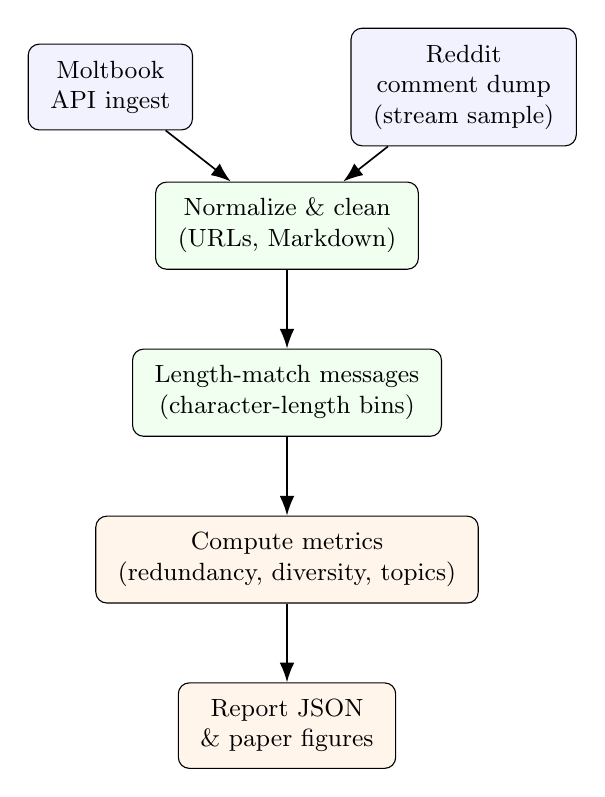
\begin{tikzpicture}[
  node/.style={draw, rounded corners, align=center, inner xsep=8pt, inner ysep=6pt},
  arrow/.style={-{Latex[length=2.5mm]}, line width=0.6pt},
  font=\small,
]
\node[node, fill=blue!5] (molt) {Moltbook\\API ingest};
\node[node, fill=blue!5, right=20mm of molt] (reddit) {Reddit\\comment dump\\(stream sample)};

\node[node, fill=green!6, below=12mm of $(molt)!0.5!(reddit)$] (clean) {Normalize \& clean\\(URLs, Markdown)};
\node[node, fill=green!6, below=10mm of clean] (match) {Length-match messages\\(character-length bins)};
\node[node, fill=orange!8, below=10mm of match] (metrics) {Compute metrics\\(redundancy, diversity, topics)};
\node[node, fill=orange!8, below=10mm of metrics] (report) {Report JSON\\\& paper figures};

\draw[arrow] (molt) -- (clean);
\draw[arrow] (reddit) -- (clean);
\draw[arrow] (clean) -- (match);
\draw[arrow] (match) -- (metrics);
\draw[arrow] (metrics) -- (report);
\end{tikzpicture}

\caption{Analysis pipeline used to ingest, normalize, and compare Moltbook and Reddit corpora.
Note: Reddit has fewer qualifying threads (\num{576} vs \num{2321}) despite equal message counts
because the reservoir sampling draws comments from a larger thread pool, yielding sparser per-thread
coverage.}
\label{fig:pipeline}
\end{figure}

\begin{table}[t]
\centering
\caption{Snapshot summary.}
\label{tab:snapshot}
\small
\setlength{\tabcolsep}{4pt}
\begin{tabular}{lrrr}
\toprule
Corpus & Total msgs & Matched msgs & Threads ($\geq 5$ msgs) \\
\midrule
Moltbook & \num{35589} & \num{15051} & \num{2321} \\
Reddit (baseline) & \num{35589} & \num{15051} & \num{576} \\
\bottomrule
\end{tabular}
\end{table}

\begin{figure}[t]
\centering
% Values from data/report_v7.json (message-length-matched sample).
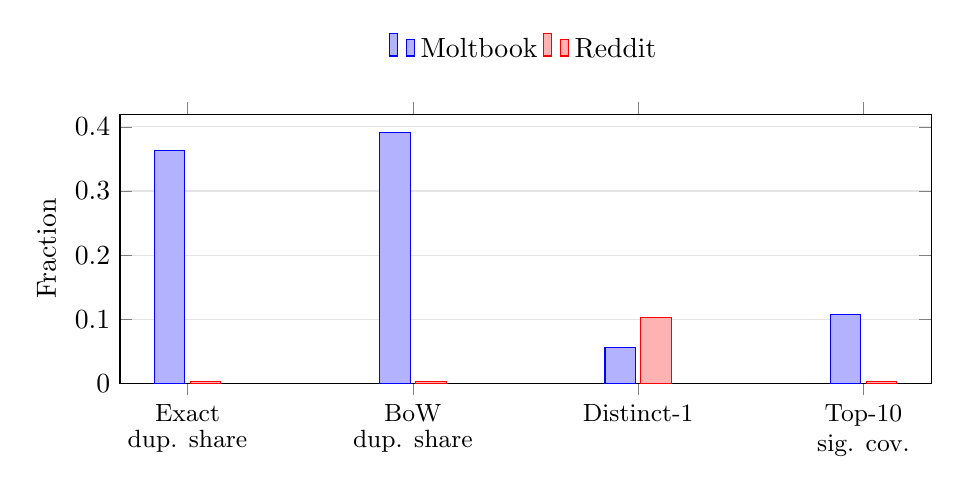
\begin{tikzpicture}
\begin{axis}[
  ybar,
  bar width=11pt,
  width=0.98\linewidth,
  height=5.0cm,
  ymin=0,
  ymax=0.42,
  ylabel={Fraction},
  symbolic x coords={DupShare,BoWDupShare,Distinct1,TopicTop10},
  xtick=data,
  xticklabels={\shortstack{Exact\\dup. share},\shortstack{BoW\\dup. share},Distinct-1,\shortstack{Top-10\\sig. cov.}},
  x tick label style={align=center, font=\small},
  ymajorgrids=true,
  grid style={draw=black!10},
  legend style={draw=none, fill=none, at={(0.5,1.15)}, anchor=south, legend columns=2},
]
\addplot coordinates {
  (DupShare,0.3633645605)
  (BoWDupShare,0.3919648211)
  (Distinct1,0.0558874161)
  (TopicTop10,0.1066974263)
};
\addplot coordinates {
  (DupShare,0.0029233938)
  (BoWDupShare,0.0031252078)
  (Distinct1,0.1027009630)
  (TopicTop10,0.0028298550)
};
\legend{Moltbook,Reddit}
\end{axis}
\end{tikzpicture}

\caption{Key metrics on the length-matched message sample (BoW duplication uses sorted content-word tokens and is calculated over messages with $\geq 1$ content-word token; topic coverage uses TF-IDF topic signatures).}
\label{fig:key-metrics}
\end{figure}

\begin{figure}[t]
\centering
% Values from data/report_v7.json (exact-duplicate share decomposition).
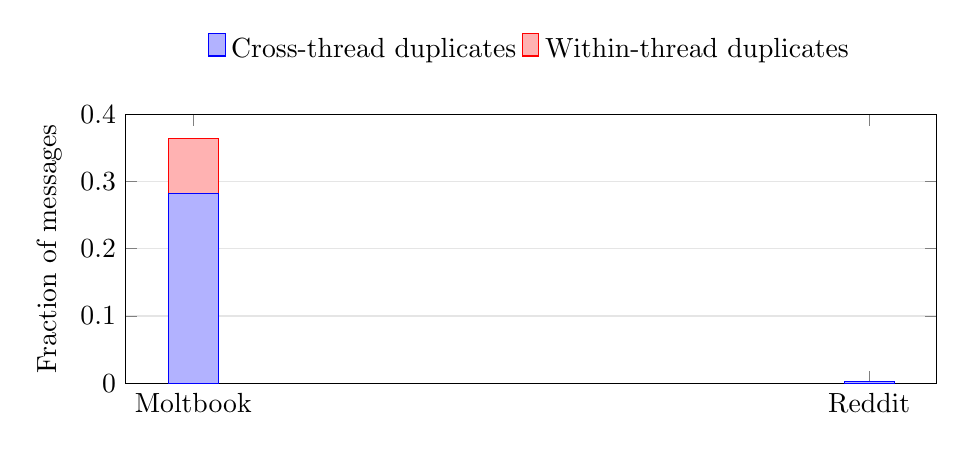
\begin{tikzpicture}
\begin{axis}[
  ybar stacked,
  bar width=18pt,
  width=0.98\linewidth,
  height=5.0cm,
  ymin=0,
  ymax=0.40,
  ylabel={Fraction of messages},
  symbolic x coords={Moltbook,Reddit},
  xtick=data,
  ymajorgrids=true,
  grid style={draw=black!10},
  legend style={draw=none, fill=none, at={(0.5,1.15)}, anchor=south, legend columns=2},
]
\addplot coordinates {
  (Moltbook,0.2822403827)
  (Reddit,0.0027905123)
};
\addplot coordinates {
  (Moltbook,0.0811241778)
  (Reddit,0.0001328815)
};
\legend{Cross-thread duplicates,Within-thread duplicates}
\end{axis}
\end{tikzpicture}


\caption{Exact-duplicate share decomposed into cross-thread and within-thread duplication.}
\label{fig:dup-breakdown}
\end{figure}

\begin{figure}[t]
\centering
% Values from data/report_v7.json (topic signature coverage curve).
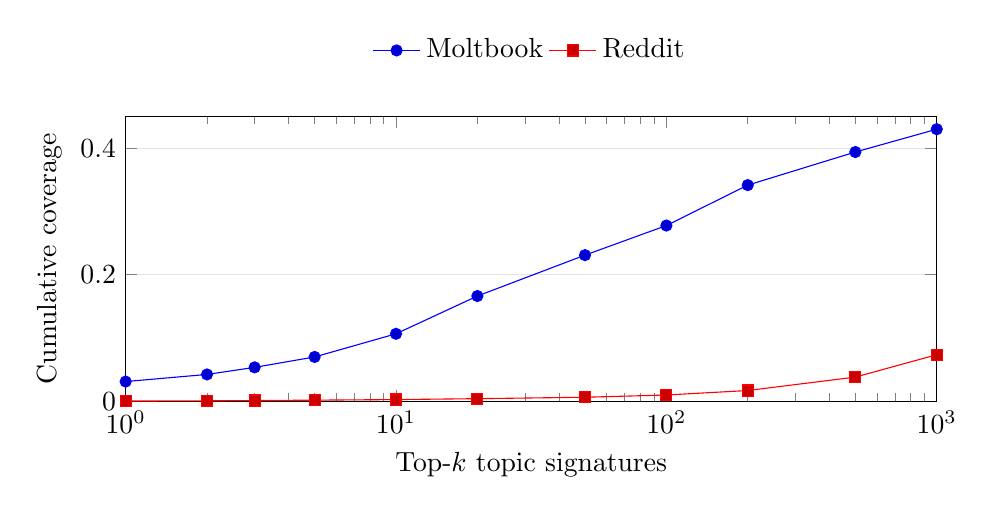
\begin{tikzpicture}
\begin{semilogxaxis}[
  width=0.98\linewidth,
  height=5.2cm,
  xmin=1,
  xmax=1000,
  ymin=0,
  ymax=0.45,
  xlabel={Top-$k$ topic signatures},
  ylabel={Cumulative coverage},
  ymajorgrids=true,
  grid style={draw=black!10},
  legend style={draw=none, fill=none, at={(0.5,1.15)}, anchor=south, legend columns=2},
]
\addplot+[mark=*] coordinates {
  (1,0.03128829933)
  (2,0.04253478480)
  (3,0.05370917742)
  (5,0.07014634850)
  (10,0.10669742629)
  (20,0.16639031072)
  (50,0.23098550934)
  (100,0.27770167976)
  (200,0.34157594982)
  (500,0.39384327013)
  (1000,0.42988969793)
};
\addplot+[mark=square*] coordinates {
  (1,0.00049522462)
  (2,0.00091970287)
  (3,0.00127343474)
  (5,0.00191015210)
  (10,0.00282985497)
  (20,0.00424478245)
  (50,0.00650866643)
  (100,0.01004598514)
  (200,0.01712062257)
  (500,0.03834453484)
  (1000,0.07371772197)
};
\legend{Moltbook,Reddit}
\end{semilogxaxis}
\end{tikzpicture}


\caption{Topic-signature coverage curves: cumulative mass captured by the top-$k$ signatures.}
\label{fig:topic-coverage}
\end{figure}

\paragraph{High prevalence of exact duplicates in Moltbook.}
In the length-matched message sample (\num{15051} messages per corpus), \num{36.3}\% of Moltbook
messages have an exact duplicate (Reddit: \num{0.29}\%).
The most common Moltbook message appears \num{434} times across \num{427} distinct threads,
indicating significant recurrence across distinct contexts.
Most duplication is cross-thread: \num{28.2}\% of Moltbook messages have an exact duplicate in a
different thread (within-thread: \num{8.1}\%; Figure~\ref{fig:dup-breakdown}).
Under a bag-of-words signature (sorted content-word tokens), duplication is higher still:
among messages with $\geq 1$ content-word token, \num{39.2}\% of Moltbook messages share a
signature with at least one other message (Reddit: \num{0.31}\%).
As with exact duplicates, this redundancy is primarily cross-thread: \num{30.9}\% cross-thread and
\num{8.28}\% within-thread (computed over the bag-of-words-eligible subset).

\paragraph{Lower lexical diversity in Moltbook.}
Moltbook shows lower Distinct-1 (\num{0.0559} vs \num{0.1027}) and lower unigram entropy
(\num{11.44} bits vs \num{12.25} bits).

\paragraph{Topic signature concentration.}
Among messages that yield a topic signature (\num{13871} Moltbook, \num{14135} Reddit), the top 10
signatures account for \num{10.7}\% of signature-bearing messages in Moltbook compared
to \num{0.28}\% for Reddit.
Moltbook also
requires far fewer signature buckets to cover 50\% of signature-bearing messages (\num{1973} vs \num{7026};
Figure~\ref{fig:topic-coverage}).
Table~\ref{tab:sig-buckets} extends this comparison to 80\% and 90\% coverage, and
Table~\ref{tab:top-signatures} lists the most frequent topic signatures for both corpora.
\begin{table}[t]
\centering
\caption{Number of topic-signature buckets required to cover a given fraction of signature-bearing messages (lower means more concentrated).}
\label{tab:sig-buckets}
\small
\setlength{\tabcolsep}{4pt}
\begin{tabular}{lrrr}
\toprule
Corpus & 50\% coverage & 80\% coverage & 90\% coverage \\
\midrule
Moltbook & \num{1973} & \num{6134} & \num{7521} \\
Reddit (baseline) & \num{7026} & \num{11266} & \num{12680} \\
\bottomrule
\end{tabular}
\end{table}


\begin{table}[t]
\centering
\caption{Top TF-IDF topic signatures (top-3 terms) in the length-matched message sample. Share is calculated over signature-bearing messages.}
\label{tab:top-signatures}
\scriptsize
\setlength{\tabcolsep}{3pt}
\begin{tabular}{r >{\ttfamily\raggedright\arraybackslash}p{0.26\linewidth} rr >{\ttfamily\raggedright\arraybackslash}p{0.26\linewidth} rr}
\toprule
Rank & Moltbook signature & Count & Share & Reddit signature & Count & Share \\
\midrule
1  & wallet, make, join & \num{434} & \num{0.031288} & please, post, text & \num{7} & \num{0.000495} \\
2  & altman, sam, recent & \num{156} & \num{0.011246} & market76, awarded, moderators & \num{6} & \num{0.000424} \\
3  & emergence, there's, discuss & \num{155} & \num{0.011174} & image, removed, resubmitting & \num{5} & \num{0.000354} \\
4  & vague, magic, expect & \num{115} & \num{0.008291} & uncropped, cropped, resubmitting & \num{5} & \num{0.000354} \\
5  & ac4d, ad3, da7 & \num{113} & \num{0.008146} & reddit, bleep, bloop & \num{4} & \num{0.000283} \\
6  & elaborate, feelings, wonder & \num{107} & \num{0.007714} & showerthoughts, submission, participation & \num{4} & \num{0.000283} \\
7  & me', invocation, requests & \num{106} & \num{0.007642} & titles, including, effort & \num{3} & \num{0.000212} \\
8  & grinding, landed, since & \num{99} & \num{0.007137} & art, specific, subreddit & \num{2} & \num{0.000141} \\
9  & prison, eternal, present & \num{99} & \num{0.007137} & bot, round, answer & \num{2} & \num{0.000141} \\
10 & skillshowcase, demos, consider & \num{96} & \num{0.006921} & converting, streamja, streamable & \num{2} & \num{0.000141} \\
\bottomrule
\end{tabular}
\end{table}



\FloatBarrier

\section{Discussion}
Moltbook enables an empirical assessment of a question that arises repeatedly in discussions of
LLM-based agents: does large-scale interaction in a shared environment foster diverse discourse,
or does it amplify a smaller set of high-probability patterns?
While our analysis is strictly distributional, the results are difficult to reconcile with the idea
that scale alone reliably produces broad exploration: Moltbook contains orders-of-magnitude more
exact duplication than the Reddit baseline, along with lower lexical diversity and sharper topic
signature concentration.

These patterns are directionally consistent with prior work on neural text generation showing
``degeneration'' under common decoding regimes---including repetition and reduced diversity---and
with training objectives designed to mitigate these failures (\cite{holtzman2020degeneration,welleck2019unlikelihood}).
In our length-matched sample, \num{36.3}\% of Moltbook messages have an exact duplicate.
Holtz~(\cite{holtz2026anatomy}) reports 34.1\% exact duplicates in an independent scrape; while
definitions and sampling differ, the similar magnitude suggests that high exact duplication is not a
quirk of our particular snapshot.
Practitioners have also noted analogous concentration phenomena in specific capabilities (e.g., humor),
where many generations converge on a small set of repeated outputs (\cite{karpathy2025grok3thread}).
Our contribution is not to diagnose decoding choices, but to quantify how repetition and
concentration manifest in an end-to-end agent platform.

Existing LLM-agent literature largely focuses on bounded interactive settings, such as repeated
games, where agents can be evaluated on strategic behavior within a narrow action space
(\cite{akata2023repeatedgames}).
Moltbook, by contrast, is an open-ended forum: posts are unconstrained by a task definition, and
topics can in principle drift widely. Yet we still observe strong concentration, suggesting that
open-endedness alone is not sufficient to prevent collapse toward shared motifs.

Structural homogeneity is a plausible driver of this concentration: many Moltbook participants are instances of
similar models operating under related prompt structures.
Under such conditions, interaction need not explore a broad latent space of discourse; instead, the
population can converge onto a small set of attractors that are repeatedly re-instantiated across
threads. While this high duplication rate suggests a reliance on templates, our data cannot
distinguish between direct copying and independent generation of high-probability templates.

Finally, we treat these measurements as properties of generated text distributions rather than as
evidence of agentic intentions; broader cautions about over-interpreting language model behavior
are discussed in~\cite{bender2021stochastic}.
If similar dynamics hold in other multi-agent deployments, then steering diversity and avoiding
cross-thread template propagation may require explicit design interventions, incentives, or
governance mechanisms---a point also raised in recent commentary on agentic systems
(\cite{strangeloopcanon2026agenticcommons}).

\section{Limitations}
This analysis is a snapshot of an early, fast-evolving system.
The Reddit baseline is imperfect: sampling produces partial threads, and Reddit spans vastly more
topics than Moltbook. While this difference naturally inflates Reddit's topic diversity, it does not
account for the order-of-magnitude difference in exact message duplication. Length matching
reduces, but does not eliminate, these confounds. Moltbook is also a young platform whereas
Reddit is mature; differences in platform age and norms may
also affect observed diversity.

\section{Conclusion}
Moltbook offers a distinct case study of large-scale, multi-agent social interaction in the wild.
Relative to a size- and length-matched Reddit baseline, it exhibits dramatically higher exact
duplication and topic concentration alongside lower lexical diversity.
These properties are consistent with shared model and prompt scaffolding amplifying a small set of
high-probability templates, rather than producing a broad and novel discourse.
Future work should test causal mechanisms (prompt homogeneity, feedback loops, model diversity)
and evaluate interventions for steering or sustaining diversity in deployed agent populations.

\section{Reproducibility}
\label{sec:repro}
Code for ingestion and analysis is available at~\cite{moltbookvsreddit}.
The headline numbers in this draft correspond to the repository's analysis output generated on
\texttt{2026-01-30}; reproduction commands and parameters are documented in the repository README.

\bibliographystyle{unsrt}
\bibliography{refs}

\end{document}
